\chapter{Background and Literature Review}
In this chapter, we explore the current research on this topic. First, by exploring the theory behind liquid neural networks, in comparison to deep neural networks. Then, by investigating popular adversarial attack methods and assessing their suitability to liquid neural network structures. Finally, current verification methods are discussed, along with their suitability to liquid neural networks. The reader should have an understanding of (traditional) neural networks and linear algebra concepts.

\section{Liquid Neural Networks}

Liquid neural networks, introduced by Ramin Hasani et al. (2021) \cite{hasaniLiquidTimeconstantNetworks2021}, are a novel class of AI algorithms, designed to maintain adaptability after completing training. These are inspired by the communication patterns of brain cells, which are flexible and responsive to new/unseen data even after their initial training phase.

Traditional neural networks use fixed architectures and static parameters, so require retraining to handle new information. Liquid neural networks use \textbf{continuous-time dynamics} to enable their state to evolve smoothly over time. This means they can dynamically adjust their responses to changing inputs during inference. This structure allows these networks to be robust against perturbations and capable of generating complex behaviors without requiring large-scale architectures.

\begin{figure}[H]
    \centering
    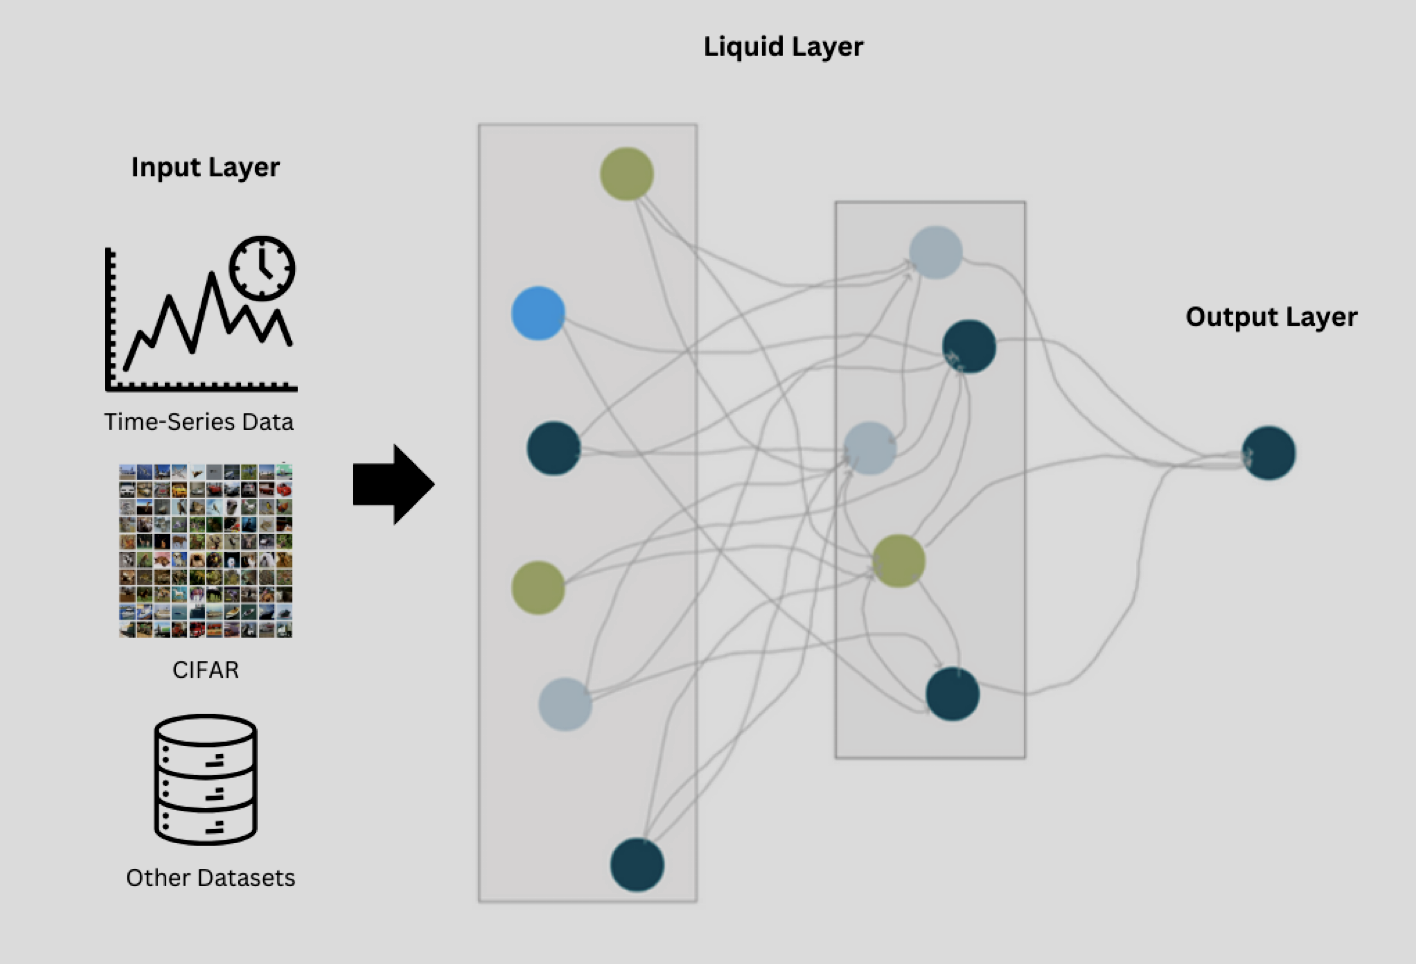
\includegraphics[width=0.7\linewidth]{img/lnn_overview.png}
    \caption{
    Schematic Diagram of a Liquid Neural Network~\cite{frank2024learning}. Figure illustrates the simplified architecture of an LNN, starting with the input layer receiving time-series data. The data then flows into the liquid layer, where dynamic, non-linear processing occurs through a complex network of interconnected neurons. Finally, the processed information is relayed to the output layer.
    }
    \label{fig:lnn_overview}
\end{figure}

LNNs use differential equations to simulate the continuous/dynamic processing and plasticity of the brain. Since LNN neurons communicate selectively with a subset of other neurons, connections formed are sparse (unlike traditional deep neural networks with dense fully-connected layers). This makes LNNs more computationally efficient than deep neural networks.

There are a range of applications of LNNs. Hasani suggests that their inherent adaptability makes them suitable for tasks requiring real-time learning and decision-making, such as autonomous driving and medical diagnosis. Their efficiency could address several challenges associated with large-scale machine learning systems, including issues related to interpretability, accountability, and environmental impact due to high carbon footprints. \cite{tedxtalksLiquidNeuralNetworks2023}

\subsection*{Continuous-Time Dynamical Systems/Differential Equations}

A \textbf{continuous-time dynamical system} is a mathematical model used to describe a system that evolves over time in a way that is continuous (rather than discrete). This means the state of the system changes smoothly as a function of time, without abrupt jumps.

In the context of liquid neural networks, the neurons' states evolve as continuous-time dynamical systems. Each neuron's state is governed by \textbf{differential equations}, enabling the network to process information dynamically and adaptively, much like physical systems in the real world. This is inspired by biological neurons, where the activity of each neuron is influenced dynamically by inputs and changes over time.

The state of each neuron \(x_i(t)\) in an LNN evolves over time according to a differential equation, expressed as:

\begin{equation} \label{eq:1}
    \frac{dx_i(t)}{dt} = f(x_i(t), u_i(t), t; \theta_i),
    \end{equation}

where:
\begin{itemize}
    \item \(x_i(t)\): The internal state of the \(i\)-th neuron at time \(t\),
    \item \(u_i(t)\): The input signal to the \(i\)-th neuron at time \(t\),
    \item \(t\): Time, treated as a continuous variable,
    \item \(\theta_i\): Trainable parameters of the neuron, such as weights and biases,
    \item \(f(\cdot)\): A function (usually nonlinear) describing the neuron’s dynamics.
\end{itemize}

A common differential equation is the \textbf{leaky integrator dynamics}, where the state evolves as:
\[
\frac{dx_i(t)}{dt} = -\alpha x_i(t) + \sum_{j=1}^N w_{ij} h(x_j(t)) + u_i(t),
\]
with:
\begin{itemize}
    \item \(-\alpha x_i(t)\): A "leakage" term causing the neuron’s state to decay over time, with \(\alpha > 0\) representing the decay rate (temporal decay),
    \item \(\sum_{j=1}^N w_{ij} h(x_j(t))\): The weighted input from other neurons, where \(w_{ij}\) is the weight from neuron \(j\) to \(i\), and \(h(x_j(t))\) is a nonlinear activation function (e.g., \(\tanh\) or ReLU),
    \item \(u_i(t)\): An external input signal.
\end{itemize}

For more complex systems, \textbf{nonlinear terms} can be included, resulting in equations such as:
\[
\frac{dx_i(t)}{dt} = g(x_i(t)) + \sum_{j=1}^N w_{ij} \sigma(x_j(t)) + u_i(t),
\]
where \(g(x_i(t))\) models intrinsic nonlinear dynamics, and \(\sigma(x_j(t))\) is a nonlinear activation function.

A liquid neural network, as a continuous-time dynamical system, has several important features. First, it ensures \textbf{smooth evolution}, where the neuron states evolve continuously over time according to differential equations. This smooth state transition is essential for modeling time-dependent values in tasks like time-series forecasting or control systems. In addition, the dynamics of the network incorporate \textbf{time dependency} \(t\) explicitly or depend solely on the current state \(x(t)\), enabling the network to capture both static and dynamic temporal relationships. Liquid neural networks are also typically \textbf{deterministic}, with their future states fully defined by the current states and inputs, but they can also accommodate \textbf{stochastic elements} to model uncertainty or noise in the environment. Finally, the network may operate under \textbf{linear} dynamics, such as \(f(x) = Ax + Bu\), which are efficient but limited in complexity, or \textbf{nonlinear} dynamics, like \(f(x) = \tanh(Wx + b)\), which allow the network to represent intricate patterns and adaptive behaviours.

\subsection*{LNN Training}
During training, the above differential equations (\ref{eq:1}) define how each neurons processes information. For each labelled training data sample, the following process occurs.

During the \textbf{forward pass}, the system of differential equations is numerically solved over time, starting from an initial state \(x(0)\). Inputs \(u(t)\) and parameters \(\theta_i\) drive the evolution of neuron states \(x_i(t)\).

The network then outputs a value, derived from the neuron states. This is compared to the target output to compute a \textbf{loss function}.

During \textbf{backpropagation through time}, gradients of the loss with respect to trainable parameters (\(\theta_i\)) are computed by differentiating through the differential equations using methods like automatic differentiation or adjoint sensitivity analysis.

Finally, \textbf{optimization algorithms} (e.g. gradient descent) update the parameters of the DEs to minimize the loss.

\subsection*{LNN Inference}
During inference, the same differential equations govern the neuron states, but parameters (\(\theta_i\)) are fixed. The network processes dynamic inputs \(u(t)\) in real-time. The equation also considers the neuron's previous state \(x_i(t)\), which is dependent on previous input values \(u(t)\). Thus, the output of each neuron is dependent on the parameters, current input values, and previously seen input values.

\subsection*{Advantages of LNNs}
Using differential equations in LNNs provides several advantages.

\subsubsection*{Temporal Modelling}
Continuous dynamics are well-suited for time-dependent tasks. This means LNNs can be used to find time-based relationships in data (temporal modeling). This form of 'memory' is highly beneficial in time-series tasks.

The nonlinear nature of \(f(x_i(t))\) ensures that the network captures complex temporal dependencies, allowing it to adjust its behavior based on the sequence and timing of inputs. This dynamic capability provides the network with a form of memory, enabling it to adapt to new scenarios even outside the training set.

This is in contrast to static models which consider data points to be independent and identically distributed.

\subsubsection*{Adaptability}
Dynamic state evolution allows the network to adapt during deployment.

The differential equation model (\ref{eq:1}) for liquid neural networks allows for state evolution even after training, resulting in increased adaptability. This is achieved by the continuous dynamics governing neuron states, which enable the network to respond dynamically to real-time inputs and changing environments.

In the DE model, \(x_i(t)\) is the state of the \(i\)-th neuron at time \(t\), \(u_i(t)\) represents external inputs, \(t\) is time, and \(\theta_i\) are trainable parameters (e.g., weights and biases). After training, the parameters \(\theta_i\) are fixed, but the neuron states \(x_i(t)\) continue to respond dynamically to new inputs \(u_i(t)\). This means the network integrates real-time inputs into its state over time, adapting its behavior dynamically to variations in the input patterns or the timing of events.

The differential equations governing the states ensure that even small variations in the input influence the system, enabling real-time adaptation.

This provides several advantages. LNNs excel in real-world scenarios involving dynamic environments, such as robotics \cite{chahineRobustFlightNavigation2023} and control systems.

For example, an LNN controlling a robotic arm in a dynamic environment would learn general principles of motion and control during training. During inference, as new obstacles appear or external forces are applied, the network integrates this new information into its state \(x_i(t)\) dynamically. This allows the robotic arm to adjust its movements in real time without needing retraining for each specific scenario.

In addition, by dynamically evolving its states, the network generalizes better to unseen data patterns by interpolating between learned behaviors.

\subsubsection*{Efficiency}
Liquid neural networks (LNNs) are inherently more efficient than traditional deep neural networks (DNNs) due to their ability to maintain sparser representations. At any given time, only a subset of an LNNs' neurons or parameters are significantly active or contribute to the system's computations. This sparsity reduces the computational overhead while retaining the network's performance and adaptability.

This is because continuous-time dynamics favor selective activity. In LNNs, neuron states evolved continuously over time, according to the differential equation \ref{eq:1}. Here \(f(\cdot)\) determines how each neuron state changes based on its inputs, past states, and parameters. The use of continuous-time dynamics enables neurons to become active only when relevant input signals \(u_i(t)\) or temporal events trigger them. This selective activity leads to fewer neurons being active at a given time, resulting in sparse representations.

LNNs are designed to work efficiently with fewer parameters compared to DNNs. While in traditional DNNs, layers are often densely connected, meaning all neurons in one layer interact with all neurons in the next layer. LNNs use sparse connectivity patterns, where neurons only interact with a limited subset of other neurons. This reflects real-world systems, such as biological brains, where neurons form selective, sparse connections.The sparsity of connections reduces the number of computations required during both training and inference.

LNNs allow the internal states of neurons to evolve over time and depend on the dynamics of the inputs. Because of this adaptability, only neurons relevant to the current input remain active. This reduces unnecessary computations and avoids the inefficiencies of global activation in traditional DNNs.

The continuous dynamics of LNNs inherently encode temporal dependencies. Unlike recurrent neural networks (RNNs) or deep learning models that require explicit mechanisms like memory gates (e.g., in LSTMs or GRUs), LNNs rely on the fluid evolution of neuron states. This reduces the overhead of managing and updating memory states, further contributing to sparsity and efficiency.

The sparse nature of LNNs offers several advantages over traditional DNNs, including reduced computational cost (minimizing matrix operations), lower energy consumption, better scalability, and robustness to overfitting (as sparse connectivity can act as a regularization mechanism by ensuring only essential features are focussed on).

\subsubsection*{Stability}
LNNs exhibit greater stability and robustness to noise compared to traditional DNNs. 

Continuous time dynamics and differential equations encode stability constraints, ensuring smooth transitions between states.

In LNNs, the state of each neuron evolves over time according to the differential equation \ref{eq:1}. The continuous nature of these equations ensures that the neuron states change gradually over time. As a result, sudden spikes in the input \(u_i(t)\) (caused by noise) are naturally smoothed out. This gradual evolution prevents abrupt changes in the neuron states, making the network less sensitive to transient noise.

In addition, neuron states evolve in response to both the current input \(u_i(t)\) and past states \(x_i(t)\). This integration over time allows the network to prioritize long-term patterns in the input and ignore temporary noise. The feedback from past states enables temporal filtering, where only meaningful input changes accumulate and influence the network’s output. In contrast, the layer-by-layer static activations in DNNs make them more susceptible to noise.

In traditional DNNs, noisy inputs can propagate through the network, often being amplified by dense connections and static parameter updates. To avoid this, special techniques can be used such as dropout. However, LNNs achieve this implicitly, by using sparse and selective connections. This limits the propagation of noise across the network. The continuous evolution of states ensures that transient noise does not significantly affect downstream neurons or outputs.

This enhanced stability has a range of benefits. LNNs perform well in real-world settings where inputs are often corrupted. The intrinsic smoothing abilities of LNNs also reduces the amount of noise-filtering preprocessing required.

\section{Adversarial Attacks}

Adversarial robustness has become a central concern in the deployment of deep learning models, particularly for safety-critical systems. Foundational studies in this area, such as those by Szegedy et al.~\cite{szegedy2013intriguing} and Goodfellow et al.~\cite{goodfellow2014explaining}, demonstrated that small, human-imperceptible perturbations can cause significant model mispredictions.

\begin{figure}[H]
    \centering
    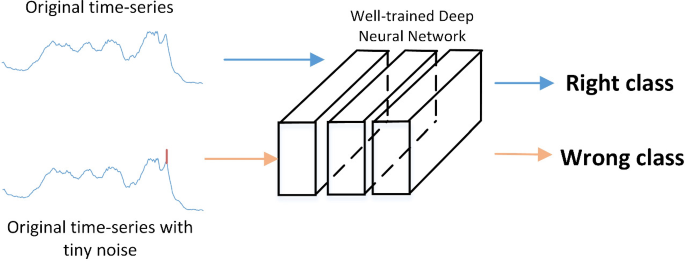
\includegraphics[width=0.7\linewidth]{img/adversarial_attack_overview.png}
    \caption{Adversarial Attack on a timeseries input~\cite{liquidTimeConstant}
\cite{liquidTimeConstant}
    }
    \label{fig:spiking2}
\end{figure}


This motivated the development of a range of attack strategies, most notably gradient-based methods like the Fast Gradient Sign Method (FGSM) \cite{goodfellow2014explaining}, its iterative counterpart PGD \cite{madry2018towards}, and more geometry-aware attacks such as DeepFool \cite{moosavi2016deepfool}. In scenarios where gradient access is limited or unavailable, black-box attacks like Simultaneous Perturbation Stochastic Approximation (SPSA) \cite{uesato2018adversarial} have proven effective.

These attack strategies have been extensively studied across various architectures including Convolutional Neural Networks (CNNs), Recurrent Neural Networks (RNNs), and Transformer-based models. Recent literature has also explored temporal robustness in sequence prediction tasks, particularly in domains such as speech \cite{cisse2017houdini}, motion tracking \cite{sun2018natural}, and control systems \cite{weng2018evaluating}.

While LNNs have demonstrated strong performance on control and robotic benchmarks, their robustness under adversarial conditions remains largely unexplored.

This project represents the first systematic exploration of adversarial vulnerabilities in Liquid Neural Networks. We evaluate the vulnerability of LNNs under a range of attack regimes, including FGSM, PGD, SPSA, and DeepFool-like variants, as well as trajectory-specific perturbations such as time-warping and continuous-time adversarial noise. While these attacks have been previously tested on discrete models like LSTMs and TCNs \cite{dong2020benchmarking}, their effects on the internal ODE solvers and state dynamics of LNNs are not well understood.

By adapting these methods to the continuous setting of LNNs and comparing the outcomes to conventional temporal models, this work provides new insights into the failure modes, dynamic vulnerabilities, and potential robustness benefits of biologically-inspired time-continuous architectures under adversarial threat.

\section{Neural Network Verification}

In this section we explore the problem of neural network verification. We look at current methods used for DNN verification, which will form the inspiration for a liquid neural network verification approach. The suitability of these to LNNs must be evaluated.

\subsection*{The Verification Problem}

Verification problems can involve concrete bounds on the input and linear programming (LP) constraints on the output. Formally, the problem can be defined as follows:

\textbf{Definition 2.2.1.1} Let \( f : \mathbb{R}^n \to \mathbb{R}^m \) be a neural network, and let \( \mathcal{X} = \{x' \in \mathbb{R}^n \mid x_i^l \leq x_i' \leq x_i^u \} \) represent the set of valid inputs constrained by the lower and upper bounds \(x^l, x^u\). Given a set of linear constraints on the output \( \psi_y \), let \( \mathcal{Y} = \{ y \mid \psi_y \} \) denote the set of outputs satisfying \( \psi_y \). The verification problem is to determine whether \( x' \in \mathcal{X} \implies f(x') \in \mathcal{Y} \), or to find a counterexample \( x' \in \mathcal{X} \) such that this implication is not true. \label{verification_def}

For input and output constraints as defined above, the goal is either to prove that no valid input violates the output constraints or to find an input that does. If no input satisfies the output constraints, we declare the property as ``safe.'' Otherwise, if such an input exists, the property is deemed ``unsafe,'' and the corresponding input serves as a counterexample. \cite {henriksenEfficientNeuralNetwork}

\subsection*{Motivation}

Verification of neural networks is a crucial problem, especially when a new architecture (such as liquid neural networks) is being researched. This is because neural networks are often deployed in safety-critical applications, such as autonomous vehicles or medical diagnosis, where unpredictability can cause significant harm. Neural networks are also vulnerable to adversarial attacks, which is when small perturbations within input data (often unnoticable to the human eye) cause significant undesired changes in the output. This vulnerability poses a serious threat to their reliability and trustworthiness. Verification ensures that the network behaves as expected under specified conditions, whilst robustness verification focuses on guaranteeing that small perturbations in the input do not lead to misclassifications or unsafe behavior. By formally proving properties of neural networks or identifying counterexamples, verification helps to ensure safety and mitigate risks in real-world deployments.

\subsection*{Symbolic and Interval Propagation Methods}

This section explores methods that focus on propagating bounds through liquid neural networks, which verifies their robustness when faced with input perturbations. \textbf{Symbolic Interval Propagation (SIP)} is a technique that computes conservative output bounds using interval arithmetic, providing a computationally efficient way to check for robustness. \textbf{CROWN (Certified Robustness to Weight Perturbations)} is more complex, and introduces linear approximations which improves the precision of robustness verification. \textbf{Lipschitz-based methods} they estimate global sensitivity by bounding the Lipschitz constant of the network. These approaches are particularly useful for ensuring scalability and efficiency, making them suitable for applications where lightweight and real-time verification is required.

\subsubsection*{SIP (Symbolic Interval Propagation)}

SIP is a scalable and efficient technique for verifying liquid neural networks by propagating symbolic intervals through the layers of the network to bound the range of possible outputs. For LNNs governed by neural ODEs with the equation \ref{eq:1}, SIP can be applied to discretize and propagate bounds over time, handling non-linearity and ensuring robustness and safety properties are satisfied under perturbations.

\paragraph{Steps in SIP:}
\begin{enumerate}
    \item \textbf{Input Interval Initialization}:
    Define the input range as intervals \([l_i, u_i]\) for each dimension \(x_i\), forming a hyper-rectangle. These intervals are represented symbolically to maintain dependencies between variables.
    
    \item \textbf{Symbolic Propagation Through Layers}:
    At each discretized time step or layer:
    \begin{itemize}
        \item \textbf{Affine Transformations}:
        For a layer \(z = W x + b\), bounds are propagated symbolically:
        \[
        l_z = W \cdot l_x + b, \quad u_z = W \cdot u_x + b.
        \]
        \item \textbf{Nonlinear Activations}:
        Nonlinearities like ReLU or \(\tanh\) are handled by updating bounds:
        \[
        \text{ReLU: } [\max(0, l_z), \max(0, u_z)], \quad
        \text{Tanh: } [\tanh(l_z), \tanh(u_z)].
        \]
    \end{itemize}
    
    \item \textbf{Output Interval Verification}:
    The final output intervals are compared against safety or robustness properties. For example, given input perturbations \(\delta x\), the output bounds \(F(x)\) must satisfy:
    \[
    F(x + \delta x) \subseteq [F_L, F_U],
    \]
    where \(F_L\) and \(F_U\) are symbolic bounds on the output.
\end{enumerate}

\paragraph{Advantages for Liquid Neural Networks}
SIP is well-suited for LNNs due to its ability to handle the continuous evolution of states in neural ODEs:
\begin{itemize}
    \item Precision: Symbolic intervals maintain variable dependencies, producing tighter bounds than traditional interval arithmetic.
    \item Efficiency: Propagation avoids the computational cost of exact methods, making SIP scalable for larger networks.
    \item Adaptability: SIP can handle nonlinear dynamics in LNNs through accurate approximations of activation functions.
\end{itemize}

\paragraph{Practical Considerations}
One consideration is over-approximation - accumulated conservativeness may reduce precision in deeper networks. Also, complex nonlinearities (within highly nonlinear layers such as softmax) require additional approximations, introducing potential conservatism. Finally, for neural ODEs, time discretization must balance accuracy with computational cost.

\subsubsection*{CROWN (Certified Robustness to Weight Perturbations)}

CROWN (Certified Robustness to Weight Perturbations) \cite{zhangEfficientNeuralNetwork2018} is a general framework for certifying the robustness of neural networks, including those with non-linear activation functions. It achieves this by bounding the outputs of the network using adaptive linear (or quadratic) upper and lower bounds for each activation function. For liquid neural networks, governed by neural ODEs, CROWN can be adapted to certify robustness by discretizing the continuous dynamics and applying its bounding technique to each time step.

CROWN provides an efficient and scalable method for verifying the robustness of LNNs. The propagated adapted bounds ensure that perturbations in the input do not lead to significant deviations in the output.

\paragraph{Mathematical Framework}
Consider a liquid neural network modeled as:
\[
\frac{dx(t)}{dt} = f(x(t), t, \theta),
\]
where \(x(t) \in \mathbb{R}^n\) is the state, \(f(x, t, \theta)\) describes the dynamics, and \(\theta\) represents the parameters. For a given perturbed input \(x_0 \in \mathbb{R}^n\) within an \(\ell_p\)-ball:
\[
x \in B_p(x_0, \epsilon) = \{x \mid \|x - x_0\|_p \leq \epsilon\},
\]
CROWN aims to compute certified bounds \(F_L(x) \leq F(x) \leq F_U(x)\), where \(F(x)\) is the output of the neural ODE after a fixed time horizon \(T\).

\paragraph{Bounding Nonlinearities}
For each activation function \(\sigma(y)\), CROWN constructs linear upper and lower bounds:
\[
h_U(y) = \alpha_U y + \beta_U, \quad h_L(y) = \alpha_L y + \beta_L,
\]
such that \(h_L(y) \leq \sigma(y) \leq h_U(y)\) over a pre-activation range \([l, u]\). These bounds are propagated through the layers of the network. For LNNs, this involves discretizing the time domain into intervals \([t_k, t_{k+1}]\) and applying the bounds iteratively at each time step.

\paragraph{Output Certification}
To certify robustness, CROWN computes bounds on the network's output \(F(x)\). Using the layer-by-layer propagation of the upper and lower bounds, the output bounds are expressed as:
\[
F_U(x) = \Lambda^{(0)} x + \sum_{k=1}^m \Lambda^{(k)} (b^{(k)} + \Delta^{(k)}), \quad
F_L(x) = \Omega^{(0)} x + \sum_{k=1}^m \Omega^{(k)} (b^{(k)} + \Theta^{(k)}),
\]
where \(\Lambda\) and \(\Omega\) are matrices representing the upper and lower bound propagation, and \(\Delta\) and \(\Theta\) account for biases introduced by non-linearities.

\paragraph{Application to Neural ODEs}
For neural ODEs, the propagation framework is adapted to account for the continuous evolution of states. The bounds are computed at each discretized step \(t_k\), ensuring that the dynamics satisfy the robustness conditions:
\[
F_U(x_0) - F_L(x_0) \geq \delta,
\]
where \(\delta\) is the minimum required margin for robustness.

\paragraph{Practical Implementation}
CROWN can be implemented as follows:
\begin{enumerate}
    \item \textbf{Define Input Bounds}: Specify the \(\ell_p\)-ball around the input \(x_0\) and initialize the pre-activation bounds for the first layer.
    \item \textbf{Propagate Bounds}: Compute the upper and lower bounds layer-by-layer using the adaptive linear approximations.
    \item \textbf{Certify Robustness}: Verify that the certified bounds at the output satisfy the desired robustness property (e.g., consistent classification).
\end{enumerate}

\subsubsection*{Lipschitz-Based Methods}

Lipschitz-based methods provide a robust framework for verifying the safety and robustness of liquid neural networks by quantifying how sensitive a network's outputs are to perturbations in its inputs. Their ability to provide global robustness guarantees is useful for neural ODEs. The Lipschitz constant of a network bounds the maximum rate at which outputs can change with respect to changes in inputs, ensuring that small input perturbations do not lead to large deviations in the output.

\paragraph{Mathematical Foundation}
For a liquid neural network modeled as:
\[
\frac{dx(t)}{dt} = f(x(t), t, \theta),
\]
where \(x(t) \in \mathbb{R}^n\) is the state, \(f(x, t, \theta)\) defines the dynamics, and \(\theta\) are the network parameters, the Lipschitz constant \(L\) satisfies:
\[
\|F(x) - F(y)\| \leq L \|x - y\|, \quad \forall x, y \in \mathbb{R}^n,
\]
where \(F(x)\) represents the solution to the neural ODE at the final time \(T\). The Lipschitz constant \(L\) bounds the global sensitivity of the network.

\paragraph{Estimation of the Lipschitz Constant}
The Lipschitz constant can be estimated for an LNN by analyzing the Jacobian of \(f(x, t, \theta)\). For a time-discretized system, the sensitivity of the network is determined by:
\[
L = \sup_{t \in [0, T]} \| J_f(x, t) \|,
\]
where \(J_f(x, t) = \frac{\partial f(x, t, \theta)}{\partial x}\) is the Jacobian matrix of \(f\). Computing or bounding \(L\) involves:
\begin{itemize}
    \item \textbf{Spectral Norm Analysis}: Evaluating \(\|J_f(x, t)\|\) as the largest singular value of the Jacobian at each time step.
    \item \textbf{Pathwise Integral Bounds}: For neural ODEs, \(L\) can be bounded using the integral of the Jacobian along the trajectory:
    \[
    L \leq \int_0^T \|J_f(x(t), t)\| dt.
    \]
\end{itemize}

\paragraph{Verification Applications}
Lipschitz-based methods are widely used for:
\begin{enumerate}
    \item \textbf{Robustness Verification}: Verifying that small input perturbations \(x_0 \to x_0 + \delta x\) result in bounded output deviations, ensuring:
    \[
    \|F(x_0 + \delta x) - F(x_0)\| \leq L \|\delta x\|.
    \]
    \item \textbf{Safety Analysis}: Ensuring the network’s outputs remain within a safe region under bounded input perturbations.
    \item \textbf{Adversarial Robustness}: Certifying that adversarial inputs cannot change the classification or decision boundaries within a certain radius.
\end{enumerate}

\paragraph{Practical Implementation}
To implement Lipschitz-based verification for LNNs:
\begin{enumerate}
    \item \textbf{Compute the Lipschitz Constant}: Use numerical methods, such as spectral norm approximation or pathwise integration, to estimate \(L\).
    \item \textbf{Bound Output Sensitivity}: Evaluate \(L\) for given input perturbations \(\delta x\) and verify that the resulting outputs satisfy safety and robustness criteria.
    \item \textbf{Scaling for Efficiency}: For high-dimensional networks, consider approximation techniques or layer-wise bounds to improve scalability.
\end{enumerate}
